\fancypagestyle{plain}{
  \fancyhf{}
  \lfoot{GOSPORT}
  \rfoot{\thepage}
  \renewcommand{\headrulewidth}{0pt}
  \renewcommand{\footrulewidth}{0.4pt}
}

\chapter{Contexte général et État de l'art} 
\minitoc

\section{Introduction}
L'essor des technologies numériques a profondément transformé de nombreux secteurs de notre société, et le domaine du sport et du bien-être n'y fait pas exception. Aujourd'hui, l'optimisation des performances athlétiques et le suivi de la santé passent inévitablement par des outils digitaux. Dans ce premier chapitre, nous mettons notre travail dans son contexte général. D’abord, nous allons présenter le contexte académique et l'organisme d'accueil. Ensuite, nous passerons en revue la problématique à l'origine de ce projet, en soulignant les défis auxquels font face les professionnels du coaching sportif. Après l'exposition de cette problématique, nous aborderons une étude détaillée de l’existant, en comparant les solutions actuelles du marché. Nous exposerons ensuite la solution proposée pour combler ces lacunes. Enfin, nous détaillerons la méthodologie de gestion de projet (Agile Scrum) ainsi que le langage de conception adoptés pour la réalisation de cette plateforme.

\section{Contexte académique et Organisme d'accueil}

\begin{figure}[H]
\centering

\includegraphics[width=4cm]{diagrams/logo-qualimetrie.png}
\caption{Logo de l'organisme d'accueil}
\end{figure}

Ce projet a été réalisé dans le cadre de notre stage de fin d'études, étape cruciale couronnant notre parcours universitaire. Ce stage a pour vocation principale de mettre en pratique l'ensemble des connaissances théoriques et techniques acquises durant notre formation académique. Il s'agit notamment de mobiliser nos compétences en développement d'applications mobiles, en conception d'architectures web distribuées, en gestion avancée de bases de données relationnelles, ainsi qu'en ingénierie logicielle globale.

Dans le cadre de ce projet académique, le travail a été mené autour de la conception et du développement de GOSPORT, une solution logicielle complète dédiée au coaching sportif et nutritionnel. L'environnement de réalisation a simulé un contexte professionnel: analyse du besoin, conception UML, développement web et mobile, intégration backend, validation fonctionnelle et préparation au déploiement.

L'immersion dans un environnement professionnel structuré nous a permis de nous confronter aux exigences réelles du monde du travail, telles que le respect des délais (deadlines), la gestion du travail en équipe, et la communication avec les différentes parties prenantes (stakeholders). De plus, ce contexte nous a offert l'opportunité de développer une application complète, robuste et évolutive, répondant à un besoin précis et avéré du marché florissant de la santé et du fitness.

\section{Problématique}
Le domaine du coaching sportif personnalisé connaît une croissance fulgurante depuis la dernière décennie. Les athlètes, qu'ils soient de haut niveau ou de simples passionnés soucieux de leur bien-être, exigent un suivi de plus en plus rigoureux, scientifique et sur-mesure pour atteindre leurs objectifs (perte de poids, prise de masse musculaire, préparation à une compétition). 

Cependant, les professionnels du coaching (préparateurs physiques, nutritionnistes, coachs personnels) font face à de multiples défis organisationnels et techniques au quotidien :

\begin{itemize}
    \item \textbf{La fragmentation extrême des outils de travail :} Aujourd'hui, un coach moyen utilise un mélange d'outils non interconnectés. Il rédige ses programmes d'entraînement sur des tableurs (Excel ou Google Sheets), il demande à ses clients d'utiliser des applications grand public pour tracker leur nutrition (comme MyFitnessPal ou FatSecret), et il communique avec eux via des messageries instantanées non professionnelles (WhatsApp, Messenger). Cette multiplication des canaux entraîne une perte d'informations critique.
    \item \textbf{Une perte de temps administratif considérable :} La consolidation des données de progression des athlètes est manuelle et fastidieuse. Le coach doit extraire les données de plusieurs plateformes pour ajuster le programme de la semaine suivante, ce qui limite considérablement le nombre de clients qu'il peut gérer simultanément de manière qualitative.
    \item \textbf{Un manque d'interactivité et de retour visuel pour l'athlète :} L'athlète reçoit généralement son programme sous un format statique (souvent un simple fichier PDF ou un tableau). Lors de sa séance en salle de sport, il n'a pas d'outil interactif pour le guider (chronomètres dynamiques, vidéos de démonstration intégrées), ce qui peut mener à une mauvaise exécution des mouvements ou à un non-respect des temps de repos, compromettant ainsi les résultats escomptés.
\end{itemize}

Face à ces constats, la question principale de notre projet de fin d'études se formule ainsi : 
\textit{Comment concevoir, modéliser et développer une plateforme numérique centralisée, multi-supports, capable de regrouper la planification complexe des entraînements, le suivi nutritionnel détaillé et la communication en temps réel entre le coach et ses athlètes, tout en garantissant une expérience utilisateur fluide, intuitive et à la pointe de la technologie ?}

\section{Étude de l’existant}
Avant d'entamer la phase de conception de notre plateforme, il est impératif d'analyser le marché actuel des applications de fitness et de coaching. Bien qu'il existe une multitude d'applications, la grande majorité cible le marché B2C (Business to Consumer), c'est-à-dire l'utilisateur final s'entraînant de manière autonome avec des programmes générés automatiquement.

Les solutions B2B (Business to Business), spécifiquement conçues pour assister les coachs dans la gestion de leurs clients, sont moins nombreuses et présentent certaines limites que nous avons analysées.

\subsection{Analyse comparative des solutions existantes}
Nous avons sélectionné trois des plateformes les plus populaires chez les professionnels du sport pour mener notre étude :

\begin{itemize}
    \item \textbf{TrueCoach :} C'est l'une des plateformes leaders du marché. Elle permet la création de programmes, le suivi vidéo et la messagerie.
    \textit{Inconvénients :} Son coût est extrêmement élevé, facturé par palier d'athlètes gérés, ce qui la rend inaccessible pour un coach débutant. De plus, son interface mobile est souvent critiquée pour son manque de modernité et son ergonomie vieillissante.
    
    \item \textbf{Trainerize :} Une plateforme très complète proposant la gestion de l'entraînement, de la nutrition et l'intégration avec des montres connectées.
    \textit{Inconvénients :} L'outil est devenu une "usine à gaz". Sa courbe d'apprentissage est très raide pour les coachs, et l'interface utilisateur est encombrée par de trop nombreuses fonctionnalités peu utilisées. L'outil ne propose pas nativement de suivi de repas macro-nutritionnel avancé sans passer par des applications tierces.
    
    \item \textbf{MyFitnessPal (Usage détourné) :} Bien que ce ne soit pas une application de coaching, de nombreux coachs exigent de leurs clients qu'ils l'utilisent pour tracker leur nourriture, puis envoient des captures d'écran.
    \textit{Inconvénients :} Aucune centralisation. Le coach n'a pas accès en temps réel au tableau de bord de son client sans partager les mots de passe.
\end{itemize}

\subsection{Tableau comparatif}

\begin{table}[H]
\centering
\renewcommand{\arraystretch}{1.5}
\resizebox{\textwidth}{!}{%
\begin{tabular}{|>{\centering\arraybackslash}p{4cm}|>{\centering\arraybackslash}p{3cm}|>{\centering\arraybackslash}p{3cm}|>{\centering\arraybackslash}p{3cm}|>{\centering\arraybackslash}p{3cm}|}
\hline
\rowcolor[HTML]{EFEFEF} 
\textbf{Fonctionnalité / Application} & \textbf{TrueCoach} & \textbf{Trainerize} & \textbf{Méthode Artisanale (Excel + WhatsApp)} & \textbf{GOSPORT (Notre Solution)} \\ \hline
\textbf{Planification d'entraînement} & Excellente & Très bonne & Bonne (mais manuelle) & Excellente \\ \hline
\textbf{Lecteur de séance interactif} & Basique & Bon & Inexistant & Très Avancé \\ \hline
\textbf{Tracker nutritionnel intégré} & Faible & Moyen & Inexistant & Excellent \\ \hline
\textbf{Messagerie temps réel}        & Oui & Oui & Oui & Oui \\ \hline
\textbf{Coût d'utilisation}           & Très onéreux (\$\$\$) & Très onéreux (\$\$\$) & Gratuit (mais coûteux en temps) & Abordable / Scalable \\ \hline
\textbf{Intégration d'Intelligence Artificielle} & Non & Faible & Non & Oui (Suggestions) \\ \hline
\end{tabular}%
}
\caption{Comparaison des solutions existantes avec GOSPORT}
\end{table}

\subsection{Bilan de l'étude de l'existant}
Ces limitations justifient pleinement la nécessité de proposer une nouvelle approche. Le marché a besoin d'un outil \textit{all-in-one} (tout-en-un), plus flexible, abordable techniquement, et qui place l'ergonomie et l'expérience utilisateur (UX) au centre du développement.

\section{Solution proposée : GOSPORT}
Afin de pallier les limites des outils existants, la solution proposée consiste à développer une plateforme technologique complète, baptisée "GOSPORT", dédiée à l'optimisation de la relation Coach-Athlète. Cette solution est conçue autour d'une architecture moderne et est composée de deux volets clients complémentaires communiquant avec un cœur de système robuste :

\begin{itemize}
    \item \textbf{L'Application Mobile (Flutter) :} Destinée principalement aux athlètes et aux coachs en déplacement. Elle est conçue pour être le compagnon de poche de l'utilisateur. Elle offre un accès immédiat aux programmes d'entraînement via un lecteur de séances immersif (Workout Player) qui gère les chronomètres de repos et valide les séries accomplies. Elle intègre également un journal de nutrition complet et une messagerie instantanée fluide. Le choix de Flutter garantit une expérience native et performante sur iOS et Android à partir d'un seul code source.
    \item \textbf{Le Tableau de bord Web (Angular) :} Conçu spécifiquement pour les coachs et les administrateurs de la plateforme. Il permet de gérer confortablement la complexité sur un grand écran : création de banques d'exercices, assignation de programmes sur plusieurs semaines via une interface calendrier (drag-and-drop), visualisation de tableaux de bord statistiques (Analytics) des progrès des athlètes.
\end{itemize}

Le système repose sur une API backend (Interface de Programmation Applicative) développée en \textbf{Node.js/Express}, un environnement reconnu pour sa très haute capacité à gérer des requêtes concurrentes de manière asynchrone. Cette API interagit avec une base de données \textbf{PostgreSQL}, un Système de Gestion de Base de Données Relationnelle (SGBDR) puissant, sélectionné pour sa robustesse, sa conformité ACID et sa capacité à gérer les relations extrêmement complexes inhérentes aux plannings d'entraînements, catalogues d'exercices et historiques de repas.

\section{Méthodologie de gestion de projet}
La conception et le développement d'un système d'information de cette envergure nécessitent une méthodologie de travail rigoureuse, permettant de s'adapter aux évolutions constantes des exigences tout en garantissant une livraison continue de valeur métier.

\subsection{Le cadre de travail Agile : Scrum}
Pour ce projet, nous avons délibérément écarté les méthodes de gestion de projet classiques (modèle en cascade ou cycle en V) au profit du cadre de travail Agile \textbf{Scrum}. Cette méthode empirique est particulièrement adaptée aux projets de développement logiciel modernes. Elle repose sur la transparence, l'inspection et l'adaptation. Elle nous permet de réévaluer rapidement les priorités, d'améliorer progressivement le produit par itérations, et de livrer des fonctionnalités exploitables régulièrement.

\begin{figure}[H]
\centering
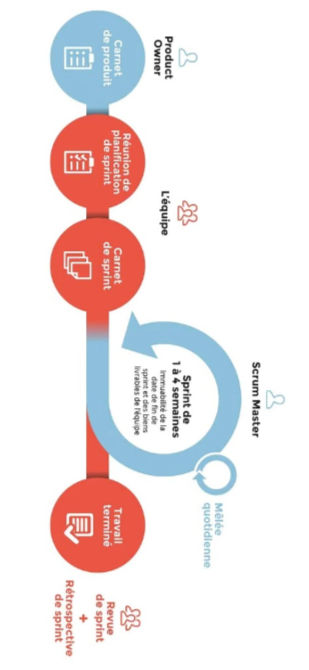
\includegraphics[width=0.7\textwidth]{diagrams/scrum.png}
\caption{Méthodologie Agile Scrum}
\end{figure}

\subsubsection{Les Rôles Scrum}
Notre équipe projet s'est organisée autour des trois rôles fondamentaux de Scrum :
\begin{itemize}
    \item \textbf{Le Product Owner (PO) :} Porteur de la vision du produit. Il est responsable de la maximisation de la valeur du produit résultant du travail de l'équipe de développement. Dans notre contexte académique, ce rôle a été simulé en collaboration avec notre encadrant, qui fixait les orientations métiers majeures.
    \item \textbf{Le Scrum Master (SM) :} Facilitateur et garant du respect du cadre Scrum. Il aide l'équipe à comprendre et à appliquer la théorie, les pratiques et les règles de Scrum, tout en levant les obstacles bloquant l'avancement.
    \item \textbf{L'Équipe de Développement (DevTeam) :} Composée de professionnels auto-organisés et pluridisciplinaires, chargés de livrer un incrément de produit fini (Done) à la fin de chaque Sprint.
\end{itemize}

\begin{table}[H]
\centering
\renewcommand{\arraystretch}{1.4}
\begin{tabular}{|l|l|}
\hline
\rowcolor[HTML]{EFEFEF} 
\textbf{Rôle Scrum} & \textbf{Personne(s)} \\ \hline
Le Product Owner & Samer Belghith \\ \hline
Le Scrum Master & Najeh Abidi \\ \hline
L'équipe de développement & Ahmed Yassine Afli / Jacem Stiti \\ \hline
\end{tabular}
\caption{Répartition des rôles du projet GOSPORT}
\end{table}

\subsubsection{Les Événements et Cérémonies Scrum}
Le processus Scrum adopté s'est articulé autour de plusieurs événements clés rythmant nos itérations de développement :
\begin{itemize}
    \item \textbf{Le Sprint :} C'est le cœur de Scrum, une boîte de temps (timebox) d'une durée fixée (généralement 2 à 3 semaines dans notre cas) pendant laquelle un incrément de produit "Terminé" et utilisable est créé.
    \item \textbf{Le Sprint Planning :} Réunion marquant le début du Sprint, où l'équipe sélectionne les éléments du Product Backlog à réaliser et définit le plan d'action (Sprint Backlog).
    \item \textbf{Le Daily Scrum :} Point de synchronisation quotidien (souvent 15 minutes) permettant à l'équipe de développement d'inspecter l'avancement vers l'objectif du Sprint et d'adapter le plan de la journée.
    \item \textbf{La Sprint Review :} Réunion en fin de Sprint pour inspecter l'incrément réalisé, présenter les démonstrations de fonctionnalités et adapter le Product Backlog si nécessaire.
    \item \textbf{La Sprint Retrospective :} Dernière étape du Sprint, dédiée à l'amélioration continue de l'équipe concernant ses processus, ses outils et ses relations humaines.
\end{itemize}

\subsubsection{Les Artefacts Scrum}
Afin d'assurer la transparence et le suivi, nous avons maintenu les artefacts suivants :
\begin{itemize}
    \item \textbf{Le Product Backlog :} La liste ordonnée et dynamique de tout ce qui pourrait être requis dans le produit final, exprimée sous forme de User Stories (récits utilisateurs).
    \item \textbf{Le Sprint Backlog :} L'ensemble des éléments du Product Backlog sélectionnés pour le Sprint en cours, assorti du plan détaillé pour créer l'incrément.
    \item \textbf{L'Incrément :} La somme de tous les éléments du Product Backlog terminés pendant un Sprint et pendant tous les Sprints précédents.
\end{itemize}

\subsection{Langage de modélisation}
Conjointement à la méthodologie Scrum, la phase de conception technique a nécessité l'utilisation d'un langage standard pour visualiser l'architecture logicielle. Nous avons opté pour le \textbf{Langage de Modélisation Unifié (UML - Unified Modeling Language)}. 

\begin{figure}[H]
\centering

\includegraphics[width=4cm]{UML.png}
\caption{Logo du Langage de Modélisation Unifié (UML)}
\end{figure}

L'UML est la norme industrielle de facto pour la spécification, la construction, la visualisation et la documentation des artefacts d'un système logiciel. Il nous a permis de représenter de manière claire, univoque et standardisée les différents aspects de "GOSPORT" :
\begin{itemize}
    \item \textbf{Aspects dynamiques et fonctionnels :} Via les \textit{diagrammes de cas d'utilisation} (pour capturer les exigences fonctionnelles des différents acteurs) et les \textit{diagrammes de séquence} (pour illustrer les interactions chronologiques complexes, telles que le flux d'authentification ou l'assignation d'un programme).
    \item \textbf{Aspects statiques et structurels :} Via les \textit{diagrammes de classes}, constituant la véritable colonne vertébrale de notre application, modélisant les entités de notre domaine métier (Coach, Athlète, Programme, Exercice) et leurs multiplicités, servant de plan direct pour l'implémentation de la base de données relationnelle.
\end{itemize}

\section{Conclusion}
Dans ce premier chapitre introductif, nous avons posé les jalons de notre projet de fin d'études. Nous avons mis en évidence les problématiques concrètes rencontrées par les professionnels du sport et proposé une solution numérique complète et ambitieuse : GOSPORT. Après avoir justifié la pertinence de notre solution face aux limites de la concurrence, nous avons détaillé l'adoption rigoureuse de la méthodologie Agile Scrum et du langage UML, garants de la réussite technique et organisationnelle du projet. Le chapitre suivant sera consacré à la phase vitale de l'analyse approfondie et à la spécification exhaustive des besoins fonctionnels et architecturaux du système.
